\chapter{Experiments} \label{chapter2}

This is a citation~\cite{utk:idr2016optimization}.
This is a very short guide to an unofficial thesis/dissertation template
for the University of Tennessee\footnote{UTK is a public university in Knoxville,
TN}.
It is based on the 2017\footnote{The 2017 template was based on a 2016 template} thesis specifications but can be easily altered
as the guidelines are changed.
This template requires a basic knowledge of \LaTeX\ and should cover
the basic requirements in terms of required packages and functionality.

\begin{figure}[!htb]
    \Centering
    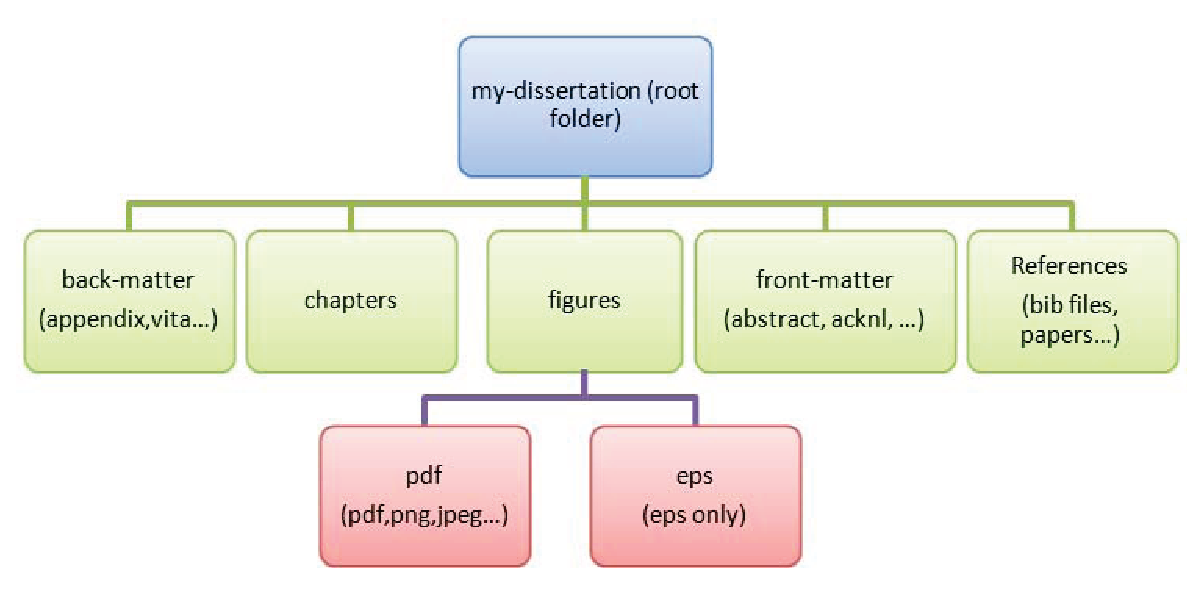
\includegraphics[width=0.9\textwidth]{fig01-folder-structure}
    \caption[UT thesis template folder structure]{UT thesis template folder structure.
        The main LaTeX file and BibTeX file are in the top directory.
        All other files are placed in any of the four folders
        (back-matter, chapters, figures, front-matter).}
    \label{fig:folderstructure2}
\end{figure}

Again, in \autoref{fig:folderstructure2} is the folder structure.

\begin{equation}
    die\ yield = wafer\ yield \times \dfrac{1}{\left(1 + \dfrac{defects\ per\ unit\ area \times die\ area}{N}\right)^N}
    \label{eq:dieyield}
\end{equation}

Use the die yield model to obtain \autoref{eq:dieyield}.

My life summary is found in \autoref{vita}.

